\chapter{Tập dữ liệu VietNamNet và tiền xử lý tiếng Việt}\label{chap:data}
\FloatBarrier
\section{Thu thập, xác minh chuyên mục và tạo tập dữ liệu}
Tập dữ liệu gồm bài VietNamNet trong 20 chuyên mục được chọn. Notebook thu thập trên tối đa 500 trang danh sách cho mỗi chuyên mục, rồi tải nội dung bằng 32 luồng xử lý song song; số 500 là giới hạn trang, không phải số bài. Một trang chứa nhiều URL, một URL có thể xuất hiện tại nhiều chuyên mục và chuyên mục ngắn kết thúc khi hết dữ liệu hợp lệ. Phạm vi này không bao phủ toàn bộ kho tin của website.

Trang danh sách dùng để phát hiện bài. Nhãn được kiểm tra trên chính trang bài, dựa vào đường dẫn chuyên mục và breadcrumb, tức chuỗi liên kết thể hiện vị trí của bài trong các mục cha--con. Tiêu đề, nội dung, URL chính thức (canonical) và bằng chứng chuyên mục được lấy cùng lượt tải HTML. Nếu thuộc chuyên mục nguồn, bài được giữ; nếu bằng chứng chỉ tới một lớp khác trong hệ thống chuyên mục, cả URL và nội dung chuyển về lớp đó. Bài ngoài hệ thống chuyên mục bị loại; lỗi tải, thiếu nội dung hoặc bằng chứng chưa đủ được thử tối đa ba lượt trước khi loại.

Mỗi nhãn có mã file ổn định. Đường dẫn Công nghiệp hỗ trợ là \texttt{hop-tac/}\allowbreak\texttt{cong-nghiep-ho-tro}, còn nhãn và tên Parquet là Công nghiệp hỗ trợ; phần đường dẫn đứng trước không tạo lớp mới. Sắc màu Việt Nam là mục con của Dân tộc -- Tôn giáo và quy về lớp cha. Không dùng mô hình đang huấn luyện để tự gán nhãn cho tập dữ liệu của chính nó: nhãn được xác định từ bằng chứng xuất bản, không từ từ khóa nội dung.

\DataTable{tables/cleaning_counts.tex}{Lượt URL, URL duy nhất và dòng văn bản là các đơn vị đếm khác nhau.}
205,463 lượt phát hiện tạo 204,280 URL duy nhất. Số bài giữ nhãn nguồn cộng số bài chuyển bằng 200,337; các nhánh còn lại gồm 3,866 bài ngoài hệ thống chuyên mục, 76 trường hợp không đạt sau ba lượt và một yêu cầu tải chuyển về địa chỉ chính thức đã có:
\begin{equation}204{,}280=199{,}463+874+3{,}866+76+1.\end{equation}
874 là số bài chuyển tính theo URL duy nhất. Thông tin mô tả quan hệ nguồn--đích có thể tính một bài ở nhiều nguồn; vì vậy, tổng ô ngoài đường chéo không thay được số bài chuyển. Trong đó có 225 quan hệ Dân tộc -- Tôn giáo tới Chính trị và 204 quan hệ Tuần Việt Nam tới Nội dung chuyên đề.
\CorpusAuditDiagram
Bản dữ liệu lưu bốn tệp JSON: raw chứa URL phát hiện, removed chứa URL bị loại hoặc gộp, meta chứa thông tin kiểm chứng, clean chứa URL theo nhãn cuối. Các tệp liên kết với nhau để truy vết một bài từ lúc phát hiện đến khi xác định nhãn cuối. Parquet giữ URL, tiêu đề, nội dung, nhãn và bằng chứng xác minh. Kiểm tra cấu trúc tệp và mã băm (hash) giúp xác nhận dữ liệu nhất quán với các quy tắc đã đặt ra. Mã băm nhận diện nội dung tệp, không chứng minh mọi nhãn đều đúng về ngữ nghĩa hoặc đã được chuyên gia gán thủ công.



\subsection{Thuật toán xác định chuyên mục cấp bài}
Chuyên mục được nhận diện theo đường dẫn (route) đã khai báo, xét đường dẫn dài trước để không chọn nhầm lớp cha khi có đường dẫn cụ thể hơn. URL được chuẩn hóa về tên miền VietNamNet hợp lệ; không lấy đường dẫn trùng tên ở một tên miền khác làm bằng chứng hệ thống chuyên mục. Canonical về cổng giảm nghèo riêng được xác định ngoài phạm vi, không ghép nhầm vào lớp chỉ vì có nội dung về vùng dân tộc.

\begin{enumerate}[leftmargin=1.6em]
\item Đọc dữ liệu có cấu trúc JSON-LD trong mã HTML trước khi trích xuất văn bản. Từ trường BreadcrumbList, thu các chuỗi chuyên mục, sắp theo thuộc tính position và đối chiếu đường dẫn với danh sách chuyên mục đã khai báo.
\item Đọc liên kết trực tiếp của breadcrumb hiển thị tại bài. Không lấy nhãn từ danh sách xổ xuống chứa toàn bộ chuyên mục của website, vì danh sách này không mô tả riêng bài đang tải.
\item Với chuỗi có thông tin ngoài mục Trang chủ (Home), lấy mục cuối khớp đường dẫn. Nếu các nguồn breadcrumb đưa ra chuyên mục khác nhau, đánh dấu chưa giải quyết để thử lại; không chọn tùy ý nguồn dễ khớp nhất.
\item Chỉ khi không có breadcrumb hữu ích, dùng trường articleSection của dữ liệu có cấu trúc nếu các tên mục quy về duy nhất một nhãn trong hệ thống chuyên mục. Trường hợp thiếu hoặc mâu thuẫn bằng chứng không được gán nhãn theo tiêu đề.
\end{enumerate}
Ba trạng thái kiểm chứng là accepted (chấp nhận), outside (ngoài phạm vi) và unresolved (chưa đủ căn cứ). Accepted cung cấp nhãn và đường dẫn bằng chứng; outside chỉ bài hợp lệ nhưng không có chuyên mục trong phạm vi; unresolved chỉ tình huống chưa đủ tin cậy để xác minh. Tải lại có thể giải quyết lỗi mạng hoặc bổ sung thông tin mô tả còn thiếu, nhưng không biến một mục ngoài phạm vi thành mục hợp lệ. Quy tắc này giúp nhãn có nguồn kiểm tra được mà không gọi toàn bộ quá trình là gán nhãn thủ công.

Các URL chuyển về cùng địa chỉ chính thức còn cần được đối chiếu nhãn trước khi gộp; nếu cùng địa chỉ có nhãn mâu thuẫn, quy trình không công bố tập dữ liệu như một bản dữ liệu hợp lệ. Trạng thái complete (hoàn tất) và mã băm chỉ được ghi nhận khi bộ tệp Parquet và danh sách URL clean đã được xuất đầy đủ. Notebook mô hình kiểm tra cấu trúc và tính nhất quán của đầu vào trước xử lý văn bản để tránh đọc một phần dữ liệu đang được xuất. Đây là bảo đảm nhất quán file, không một kết luận về đúng sai ngữ nghĩa.


\subsection{Đơn vị quan sát và chất lượng nhãn}
Nhãn nguồn của trang danh sách và nhãn cuối của bài là hai thuộc tính khác nhau. Giữ liên kết nguồn cho phép giải thích vì sao bài được chuyển lớp, nhưng chỉ nhãn xác minh mới là mục tiêu giám sát. Tương tự, các yêu cầu tải từ những URL khác nhau có thể chuyển hướng về cùng địa chỉ chính thức. Gộp các URL này khác với phát hiện bài có văn bản trùng nhau. Đếm URL duy nhất chưa loại được hai địa chỉ có cùng nội dung, nên còn cần bước xử lý ở tập dữ liệu văn bản.

Chính sách nhãn cha--con chỉ áp dụng cho các nhánh chuyên mục đã xác định; không suy ra mọi chuyên mục chứa từ ``dân tộc'' đều phải về cùng một lớp. Các mục Dân tộc -- Tôn giáo và Dân tộc thiểu số và miền núi giữ hai ID riêng trong hệ thống chuyên mục. Cách tổ chức này có thể tạo bài gần về ngữ nghĩa nhưng khác nhãn tham chiếu; phần đánh giá cần phản ánh cả hai nhãn chứ không âm thầm gộp chúng để tăng điểm.

Không đạt sau các lần thử lại là nhóm không đủ điều kiện tạo bản ghi, chưa nhất thiết là một bài chắc chắn ngoài hệ thống chuyên mục. Bảng đếm giữ các lý do riêng để tránh coi lỗi mạng hoặc thiếu nội dung như một quyết định chủ đề. Việc loại nhóm này cũng có thể làm bản dữ liệu thiên lệch theo khả năng tải và trích xuất. Những bài đã tải tốt không tạo bằng chứng về chất lượng trên toàn bộ lịch sử xuất bản.

\FloatBarrier
\section{Phân bố nhãn, mất cân bằng và chia tập}
Sau khi chuẩn hóa văn bản, các bản ghi có cùng văn bản được gom thành nhóm. Tám bản ghi thuộc nhóm có nhãn mâu thuẫn bị loại; với các nhóm cùng nhãn, chỉ giữ một đại diện và bỏ 364 bản ghi lặp. Tập dữ liệu còn 199,965 bài. Bảng~\ref{tab:class_split} đối chiếu số bài trong Parquet đầu vào với số bài còn lại sau bước này. Phép chia phân tầng dùng tỷ lệ 70/15/15 và seed 42, tạo 139,975 bài huấn luyện, 29,995 bài xác thực và 29,995 bài kiểm tra. Cách chia này giữ tỷ lệ các lớp gần phân bố tập dữ liệu; chênh một mẫu giữa validation/test là hệ quả làm tròn số lượng nguyên.
\begin{table}[htbp]\centering\small\setlength{\tabcolsep}{3pt}
\caption{Hệ thống chuyên mục và số bài ở từng giai đoạn; ID thống nhất trong notebook và app.}\label{tab:class_split}
\begin{tabularx}{\linewidth}{r>{\raggedright\arraybackslash}Xrrrrr}
\toprule
ID & Chuyên mục & Parquet & Sau khử trùng & Train & Val & Test\\\midrule
0 & Bạn đọc & 12.310 & 12.119 & 8.483 & 1.818 & 1.818\\
1 & Bất động sản & 12.311 & 12.309 & 8.616 & 1.847 & 1.846\\
2 & Chính trị & 12.243 & 12.242 & 8.569 & 1.837 & 1.836\\
3 & Công nghiệp hỗ trợ & 1.297 & 1.292 & 905 & 193 & 194\\
4 & Công nghệ & 11.062 & 11.061 & 7.743 & 1.659 & 1.659\\
5 & Du lịch & 10.980 & 10.979 & 7.685 & 1.647 & 1.647\\
6 & Dân tộc - Tôn giáo & 3.700 & 3.700 & 2.590 & 555 & 555\\
7 & Dân tộc thiểu số và miền núi & 1.088 & 1.088 & 762 & 163 & 163\\
8 & Giáo dục & 12.261 & 12.259 & 8.581 & 1.839 & 1.839\\
9 & Kinh doanh & 12.649 & 12.643 & 8.850 & 1.896 & 1.897\\
10 & Nông thôn mới & 969 & 969 & 678 & 145 & 146\\
11 & Nội dung chuyên đề & 12.569 & 12.568 & 8.798 & 1.885 & 1.885\\
12 & Sức khỏe & 12.385 & 12.385 & 8.670 & 1.858 & 1.857\\
13 & Thế giới & 11.889 & 11.889 & 8.322 & 1.783 & 1.784\\
14 & Thể thao & 12.401 & 12.267 & 8.587 & 1.840 & 1.840\\
15 & Thời sự & 12.420 & 12.420 & 8.694 & 1.863 & 1.863\\
16 & Tuần Việt Nam & 11.280 & 11.276 & 7.893 & 1.692 & 1.691\\
17 & Văn hóa - Giải trí & 12.318 & 12.317 & 8.622 & 1.848 & 1.847\\
18 & Ô tô - Xe máy & 12.300 & 12.299 & 8.609 & 1.845 & 1.845\\
19 & Đời sống & 11.905 & 11.883 & 8.318 & 1.782 & 1.783\\
\bottomrule\end{tabularx}
\end{table}
\SplitDiagram
\ReportFigure[.94]{assets/compact/class_distribution_final.png}{Phân bố 20 lớp của tập dữ liệu cuối 199,965 bài, sau khi bỏ bài trùng lặp nội dung.}
Kinh doanh có 12,643 bài, Nông thôn mới 969 bài; hai lớp Dân tộc thiểu số và miền núi, Công nghiệp hỗ trợ lần lượt có 1,088 và 1,292 bài. Nhiều lớp lớn có số lượng gần nhau do phạm vi phân trang, không phải do lấy mẫu ngẫu nhiên từ toàn bộ báo. Tỷ lệ lớn/nhỏ và trọng số train vì thế cần được đọc trong bản dữ liệu này: tỷ số giữa trọng số lớp lớn nhất và nhỏ nhất trong tập huấn luyện khoảng 13.05 lần.

Accuracy chịu ảnh hưởng nhiều hơn từ các lớp đông; Macro-F1 dành đóng góp ngang nhau cho mỗi lớp. Tuy nhiên, ít mẫu không phải nguyên nhân đơn độc của chất lượng thấp. Công nghiệp hỗ trợ có ít bài nhưng tín hiệu chủ đề tập trung; các lớp giao thoa có thể khó ngay cả khi số mẫu lớn. Phân tích thực nghiệm sẽ đối chiếu số lượng với precision/recall và hướng nhầm, thay vì mặc định tăng trọng số lớp giải quyết mọi lỗi.


Phân tầng giữ mỗi lớp trong ba tập; nó không làm cân bằng số mẫu giữa các lớp. Do đó, tập test vẫn thể hiện lớp Nông thôn mới nhỏ hơn nhiều lớp lĩnh vực, và tỷ lệ đúng tổng bị chi phối bởi các chuyên mục đông hơn. Đây là lý do dùng cả chỉ số tổng và theo lớp, thay vì oversample test để tạo một mức Accuracy dễ nhìn hơn.

Các nhãn bình luận và chuyên đề không chỉ khác nhau ở số lượng. Chúng có thể chứa từ vựng của lĩnh vực đang được bàn tới, khiến hai bài tương tự về chủ đề mang chuyên mục khác nhau. Trong thiết kế đầu vào không dùng URL/breadcrumb, bộ phân loại phải suy quyết định biên tập chỉ từ văn bản. Một phần độ khó vì vậy thuộc cách định nghĩa mục tiêu, không thể quy hết cho kích thước train.
\FloatBarrier
\section{Ghép văn bản, chuẩn hóa và phân đoạn từ}
Tập dữ liệu chung ghép tiêu đề, một khoảng trắng và nội dung, với tiêu đề xuất hiện một lần. Thứ tự xử lý là chữ thường, thay ký tự ngoài \texttt{\textbackslash w,\textbackslash s}, bỏ chuỗi chữ số, PyVi và thu gọn khoảng trắng. Dấu tiếng Việt trong Unicode thông thường được giữ; dấu gạch dưới biểu diễn một từ nhiều âm tiết. Stopwords được giữ ở tập dữ liệu chung. SVM/LR loại từ dừng và lặp tiêu đề thêm hai lần sau khi chốt tập dữ liệu và chia tập.
\PreprocessDiagram
\DataTable{tables/preprocessing_example.tex}{Trích đoạn UNIQLO từ output thật; ba trạng thái thể hiện thay đổi chữ số, dấu câu và đơn vị từ.}
Khoảng trắng tiếng Việt có thể phân cách âm tiết chứ chưa phải từ. PyVi nối các âm tiết thành đơn vị như \texttt{trẻ\_em}, \texttt{thiên\_tai} \citep{pyvi}. BPE là bước tiếp theo riêng của tokenizer PhoBERT: một đơn vị PyVi có thể gồm nhiều subword. Đơn vị từ, khoảng trắng và vị trí BPE không được dùng thay nhau khi đo chiều dài hay thiết kế cắt ngắn đầu vào.

Chữ thường làm mất case của tên riêng; loại chữ số làm mất năm, giá và số hiệu; thay dấu câu làm mất một phần ranh giới câu. Chưa có ablation xác nhận từng bước đều cải thiện F1. Quy trình phân loại không có bước NFC riêng, nên không cam kết bảo toàn mọi chuỗi Unicode có dấu tổ hợp. PhoBERT được tiền huấn luyện với phân đoạn của VnCoreNLP, trong khi thực nghiệm và app dùng PyVi \citep{phobert,phobertcard,vncorenlp2018}; sự nhất quán huấn luyện/suy luận chưa loại bỏ khác biệt với tiền huấn luyện.

\FloatBarrier
\section{Độ dài đầu vào và tác động của giới hạn token}
Bảng~\ref{tab:lengths} nêu rõ giai đoạn tập dữ liệu và đơn vị đo. Trung vị là mốc chia đôi số bài theo độ dài; P95 là mốc mà 95\% số bài không vượt quá. Các thống kê trước khi bỏ bài trùng lặp không được coi như số mẫu của tập dữ liệu cuối; số ký tự nội dung cũng khác số từ của chuỗi ghép tiêu đề--nội dung. P95 của các hàng sau khi bỏ bài trùng lặp được tính từ mảng độ dài đã xuất, không cần chạy lại tokenizer.
\begin{table}[htbp]\centering\small\caption{Chiều dài ở các mức biểu diễn và bản dữ liệu. Dấu -- là thống kê không dùng tại đây.}\label{tab:lengths}
\begin{tabularx}{\linewidth}{>{\raggedright\arraybackslash}Xlrrr}\toprule Văn bản / giai đoạn & Đơn vị & Trung bình & Trung vị & P95\\\midrule
Tiêu đề; trước khi bỏ bài trùng lặp & Đơn vị cách trắng & 14.26 & 15 & --\\
Nội dung; trước khi bỏ bài trùng lặp & Đơn vị cách trắng & 693.28 & 617 & --\\
Nội dung; tập dữ liệu cuối & Ký tự & 3,198.85 & 2,840 & 6,645\\
Tiêu đề + nội dung; tập dữ liệu cuối & Từ PyVi & 524.16 & 465 & 1,090\\
Mẫu BPE 1,000 bài & Subword + token đặc biệt & 572.973 & 510.5 & 1,169.35\\\bottomrule\end{tabularx}
\end{table}
Khảo sát BPE trên 1,000 bài, seed 42, tính cả token đặc biệt: trung bình 572.973, trung vị 510.5; 85.4\% vượt 256 token. Head--Tail giữ trung bình 56.32\% token nội dung trong mẫu này. Các tỷ lệ không đo phần ngữ nghĩa được bảo toàn và không phải một lần đếm toàn bộ tập dữ liệu.
\begin{figure}[tbp]\centering
\begin{subfigure}[t]{.48\textwidth}\centering
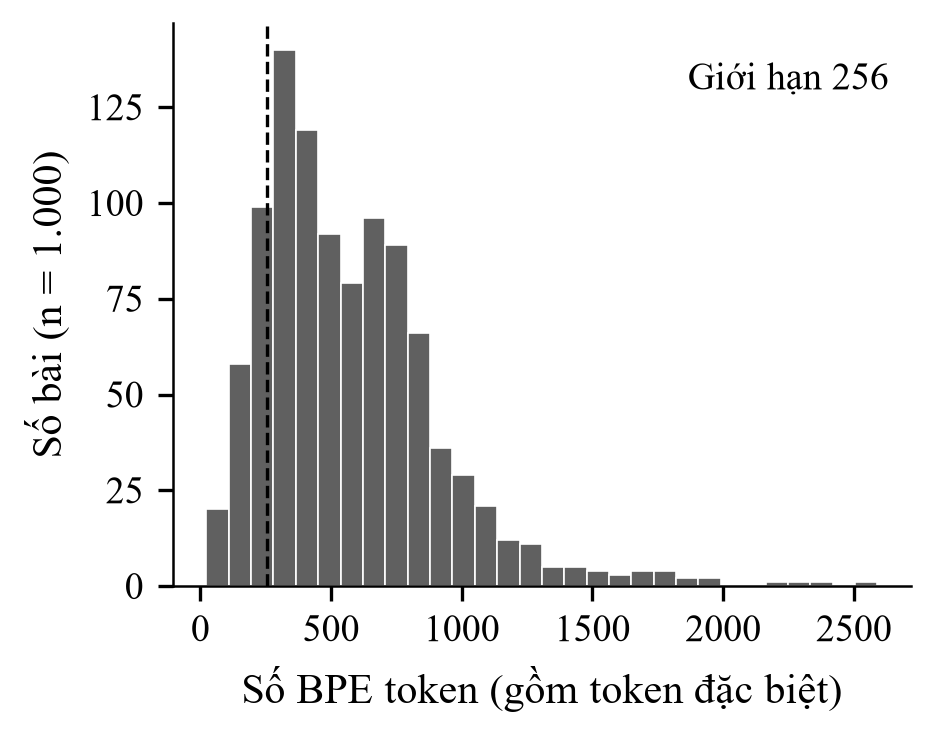
\includegraphics[width=\linewidth]{assets/compact/bpe_length.png}\caption{Độ dài BPE, gồm token đặc biệt.}\end{subfigure}\hfill
\begin{subfigure}[t]{.48\textwidth}\centering
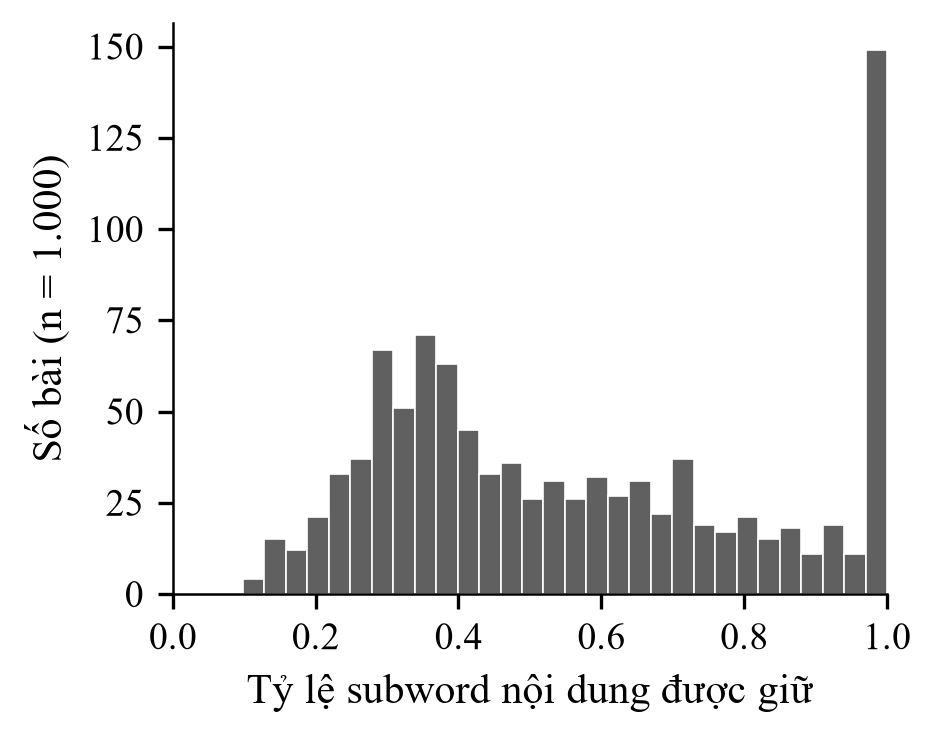
\includegraphics[width=\linewidth]{assets/compact/bpe_retention.png}\caption{Tỷ lệ subword nội dung được giữ.}\end{subfigure}
\caption{Khảo sát 1,000 bài: giới hạn 256 vị trí làm mất một phần đáng kể chuỗi đầu vào.}\label{fig:bpe-length-retention}\end{figure}
BiLSTM giới hạn 512 từ PyVi; trên tập dữ liệu cuối, 44.14\% bài vượt độ dài này và tỷ lệ từ giữ trung bình là 87.13\%. Hai kết quả không trực tiếp so với 56.32\% của PhoBERT: khác đơn vị, phạm vi khảo sát và tokenizer. SVM/LR dùng toàn văn nhưng nén văn bản thành vector thưa, làm mất thứ tự xa. Mỗi hướng giữ và bỏ loại thông tin khác nhau.


Một tỷ lệ giữ cao ở mức token chưa chứng minh những đoạn quyết định nhãn đã được giữ. Chẳng hạn, thông tin chủ đề có thể lặp ở mở đầu, hoặc chỉ rõ ở phần giữa bị cắt; thống kê chiều dài không phân biệt hai trường hợp. Ngược lại, bỏ một phần lớn token không nhất thiết làm mất tương ứng từng đó tín hiệu nếu bài chứa lặp và đoạn phụ. Báo cáo dùng thống kê để xác định mức độ phổ biến của cắt ngắn đầu vào, không đổi nó thành một ước lượng mất ngữ nghĩa.

\FloatBarrier


Nội dung dài nhất trong mảng tập dữ liệu có 131,081 ký tự, còn chuỗi chuẩn hóa dài nhất có 20,547 từ PyVi. Các cực trị cho thấy không thể giả định mọi bài nằm gần giá trị trung bình hoặc trung vị. Chúng cần được rà soát theo bài để phân biệt nội dung dài thật, đoạn liên quan và lỗi trích xuất. Báo cáo không dùng cực trị để suy một giới hạn cắt mới chưa được thử trên validation.

Giới hạn chuỗi tác động vào vị trí, còn từ vựng tác động vào kiểu token. BiLSTM có thể giữ đủ độ dài một bài nhưng vẫn thay từ lạ bằng UNK; PhoBERT có thể biểu diễn từ lạ bằng nhiều subword nhưng vì thế sớm đạt giới hạn 256 hơn. TF--IDF dùng toàn bài, song từ không thuộc từ vựng train hoặc bị bộ lọc số tài liệu chứa từ loại sẽ không có chiều riêng. Mỗi cơ chế mất thông tin khác nhau, nên ``không cắt bài'' không đồng nghĩa giữ toàn bộ thông tin văn bản.

Khảo sát BPE dùng mẫu cố định 1,000 bài giúp tái kiểm tra biểu đồ phân bố và tỷ lệ giữ mà không mã hóa lại tập dữ liệu. Kết quả phải đi cùng cỡ mẫu và seed, trong khi phân bố lớp/split dùng toàn tập dữ liệu cuối. Một biểu đồ mẫu có thể mô tả độ dài phổ biến nhưng chưa đại diện từng lớp ít bài với độ chính xác như toàn bộ mẫu. Khi đánh giá tác động cắt ngắn đầu vào theo nhãn, cần một phân tích có số mẫu và độ bất định riêng.


\section{Loại bỏ bài trùng lặp, phòng ngừa rò rỉ dữ liệu và giới hạn dữ liệu}
Nếu nhiều bản ghi có văn bản giống nhau sau chuẩn hóa nhưng nhãn khác nhau, cả nhóm bị loại thay vì tùy chọn một nhãn. Dòng lặp cùng nhãn được giữ một đại diện. Quy tắc này áp dụng trước khi chia tập, bỏ từ dừng và tăng trọng số tiêu đề, để bốn quy trình phân loại dựa trên cùng tập bài chứ không có bốn tập dữ liệu khác nhau do cách tạo đặc trưng.

Chín phép đối chiếu giữa ba tập theo URL, văn bản thô và văn bản chuẩn hóa không phát hiện giao nhau chính xác. Từ vựng BiLSTM và từ vựng/IDF TF--IDF chỉ học từ tập huấn luyện; validation/test dùng các biến đổi cố định. Đối chiếu mã băm trùng khớp chưa đánh giá bài viết lại, gần trùng hoặc nhiều bài về cùng sự kiện. Phép chia ngẫu nhiên cùng nguồn vì vậy không mô phỏng đầy đủ dự đoán tin tương lai.

Bộ nhớ đệm (cache) lưu kết quả xử lý để có thể dùng lại mà không tính toán từ đầu. Cache có mã nhận diện dữ liệu gắn bản dữ liệu, mapping, split và biểu diễn; số dòng bằng nhau chưa đủ để tái sử dụng cache. Mỗi notebook mô hình có cache riêng, không tham gia quá trình thực thi của app. Bản dữ liệu có thể còn quảng bá, đoạn liên quan hoặc nhiễu trích xuất, chưa được kiểm toán ngữ nghĩa toàn bộ. Dữ liệu sạch được hiểu là đạt quy tắc xác minh và kiểm tra đã công bố; đường dẫn tái hiện được tập trung tại Phụ lục~\ref{app:evidence}.
